\begingroup %{
\newcommand{\bou}{{\,|\,}}
\newcommand{\boug}{{\,\big|\,}}
\newcommand{\bougg}{{\,\bigg|\,}}
\newcommand{\word}[1]{{|\!\lfloor{#1}\rfloor\!|}}
{\setlength\arraycolsep{2pt}
%
\section{On Fixed Point Equations over Commutative Semirings}\label{s1:EKL07} %{
	\cite{EKL07}のノートを書いておく。\cite{EKL07}は、\cite{Hopkins99}での
	ベキ等半環に対する議論を、$\omega$-連続な半代数に対するものに拡張している。

\subsubsection{$\omega$-連続}\label{s3:オメガ-連続} %{
	\begin{itemize}\setlength{\itemsep}{-1mm} %{
		\item 自然な順序 \\
		半環$R$に次の半順序$\le$が定義できるとき、$\le$を自然な順序という。
		\begin{equation*}\begin{split}
			r_1\le r_2 \iff \text{ there exists } s\in R \text{ such that } 
			r_1 + s = r_2
		\end{split}\end{equation*}
		自然数には自然な順序が定義できるが、整数には自然な順序が定義できない。
		\item $*$-完備 \\
		任意の$R$の元に対してKleeneスターが定義できると仮定する。
		$1^*=\sum_{n\in\sizen}1\not\in\sizen$だから自然数は$*$-完備でないが、
		自然数に無限大を付け加えたものは$*$-完備になる。
		\item $\omega$-連続 \\
		自然な順序が定義され、$*$-完備であり、任意の$n\in\sizen$に対して
		$r_n\in R$ならば、$\sum_{n\in\sizen}r_n\in R$となる。
		$*$-完備はKleeneスターが収束することを要求するが、$\omega$-連続は、
		もっと強く、任意の可算和が収束することを要求する。非常に強い要請で、
		通常扱う半環では満たされない。
		自然数に無限大を付け加えたものは$\omega$-連続になる。
		わかった気がしない。\cite{esik2007modern}に$\omega$-連続のチャンとした
		定義があるので、読むしかないようだ。
	\end{itemize} %}
%s3:オメガ-連続}

\subsubsection{逐次近似たち}\label{s3:逐次近似たち} %{
	\begin{itemize}\setlength{\itemsep}{-1mm} %{
		\item Kleeneの逐次近似 \\
		$\omega$-連続な半環上の任意の形式級数$f$に対して、
		$x=\plr{f\bou x}$の最小不動点$\lim_{n\to\infty}x_n$は存在する。
		\begin{equation*}\begin{split}
			x_0 &= 0 \\
			x_1 &= \plr{f\bou x_0} \\
			\vdots \\
			x_{n+1} &= \plr{f\bou x_n} \\
		\end{split}\end{equation*}
		ここで、今考えている係数環は$\omega$-連続であることに注意する。
		例えば、自然数に無限大を付け加えたものであり、無限大も含めれば解がある
		と言っている。通常の意味、有限の範囲内、では、解が存在するとは限らない。
		$\omega$-連続では、二本の直線は必ずどこかで交わるという、球面上の幾何
		のようなことが起きる。無限大を付け加えることは、Poincare写像による直線
		の完備化と同等なことからもわかる。
		この逐次近似が最小不動点を与えることの証明は、Wikipedia
		\url{http://en.wikipedia.org/wiki/Kleene_fixed-point_theorem}にある。
		\begin{itemize}\setlength{\itemsep}{-1mm} %{
			\item 半順序集合$R:=(R,\le)$で、次の性質を満たす
			$\plr{f\bou x}\in R\bblr{x}$をモノトーンという。
			\begin{equation*}\begin{split}
				x\le y\in R \implies \plr{f\bou x}\le \plr{f\bou y}
			\end{split}\end{equation*}
			%
			\item $R$が最小値$\bot$を持つ時、$\plr{f\bou x}\in R\bblr{x}$を
			モノトーンとすると、次の式が成り立つ。
			\begin{equation*}\begin{split}
				\bot\le \plr{f\bou\bot}\le \plr{f^{\circ2}\bou\bot}
				\le \plr{f^{\circ3}\bou\bot}\le\cdots
			\end{split}\end{equation*}
			$f$の次数による帰納法で証明できる。$\bot$が最小値だから、
			$\bot\le \plr{f\bou\bot}$が成り立ち、次の式が成り立つ。
			\begin{equation*}\begin{split}
				\plr{f^{\circ n}\bou x}\le \plr{f^{\circ\plr{n+1}}\bou x}
				&\implies f\plr{f^{\circ n}\bou x}\le f\plr{f^{\circ\plr{n+1}}\bou x} \\
				&\iff \plr{f^{\circ\plr{n+1}}\bou x}\le \plr{f^{\circ\plr{n+2}}\bou x}
			\end{split}\end{equation*}
			%
			\item さらに、$R$では、任意の増大列$r_0\le r_1\le\cdots\in R$が収束
			すると仮定すると(directed complete partial orders)\footnote{
				directed complete partial ordered setを日本語に訳すと、
				有向完備半順序集合となるそうだが、とても覚えられそうにない。
			}、
			$\set{f^{\circ n}\bou n\in\sizen}$は最大元$f^\top\in R$を持つ。
			\begin{equation*}\begin{split}
				f^\top := \sup f_\bot^* \quad\text{where }
				f_\bot^* := \set{\plr{f^{\circ n}\bou\bot}\bou n\in\sizen} \subseteq R
			\end{split}\end{equation*}
			%
			\item さらに、$f$が次の性質を満たせば(Scrott-連続)、
			\begin{equation*}\begin{split}
				\plr{f\bou \sup A} = \sup\plr{f\bou A}
				\quad\text{for all } A = \set{a_0\le a_1\le\cdots\in R}
			\end{split}\end{equation*}
			次の式から$f^\top$が$f$の不動点になることがわかる。
			\begin{equation*}\begin{split}
				f^\top = \sup f_\bot^* = \sup f_\bot^+ = \sup \plr{f\bou f_\bot^*}
				= \plr{f\bou \sup f_\bot^*} = \plr{f\bou t^\top}
			\end{split}\end{equation*}
			%
			\item すると、$f^\top$が$f$の最小不動点になることがわかる。
			このことは、$f_\bot^*$の任意の元が、任意の$f$の最小不動点より
			小さいことを示せばよい。帰納法で証明する。$r\in R$を$f$の不動点とする。
			$\bot\le r$が成り立ち、ある$n\in\sizen$で$\plr{f^{\circ n}\bou\bot}\le r$が成り立つとすると、
			$\plr{f^{\circ\plr{n+1}}\bou\bot}\le\plr{f\bou r}=r$となる。
		\end{itemize} %}
		%
		\item Newtonの逐次近似 \\
		cc-半環上の任意の形式級数$f$に対して、
		$x=\plr{f\bou x}$の最小不動点$\lim_{n\to\infty}x_n$は存在する。
		\begin{equation*}\begin{split}
			x_0 &= 0 \\
			x_1 &= \plr{f\bou x_0} + \plr{\partial f\bou x_0}\plr{x_1 - x_0} \\
			\vdots \\
			x_{n+1} &= \plr{f\bou x_n} + \plr{\partial f\bou x_n}\plr{x_{n+1} - x_n} \\
		\end{split}\end{equation*}
		漸化式は次のように書き換えることができる。
		\begin{equation*}\begin{split}
			x_{n+1} = \frac{\plr{f\bou x_n} - \plr{\partial f\bou x_n}x_n}
			{1 - \plr{\partial f\bou x_n}}
			= x_n + \frac{\plr{f\bou x_n} - x_n}{1 - \plr{\partial f\bou x_n}}
		\end{split}\end{equation*}
		Newtonの逐次近似の場合、$\plr{\partial f\bou x_n} = 1$となる点$x_n$が
		あると、漸化式を進めることができなくなる。この時には、
		$\plr{f\bou x_n}=x_n$でない限り、漸化式が破綻する。
		また、実数の場合は、無限ループに入ることあるようだ。cc-半環でも
		無限ループに入ることがあるのだろうか?
		%
		\item Hopkins-Kozenの公式 \\
		ベキ等なcc-半環上の任意の形式級数$f$に対して、
		$x=\plr{f\bou x}$の最小不動点$x_1$は存在して、
		次のように与えられる。
		\begin{equation*}\begin{split}
			x_0 &= \plr{f\bou 0} \\
			x_1 &= x_0 + \plr{f\bou x_0}x_1
		\end{split}\end{equation*}
	\end{itemize} %}

	ベキ等半環の場合、次の式が成り立ち、
	\begin{equation*}\begin{split}
		\plr{f\bou x} - \plr{\partial f\bou x}x = \plr{f\bou 0}
	\end{split}\end{equation*}
	次のように、Newtonの逐次近似からHopkins-Kozenの逐次近似が導かれる。
	\begin{equation*}\begin{split}
			x_{n+1} 
			&= \plr{f\bou x_n} + \plr{\partial f\bou x_n}\plr{x_{n+1} - x_n} \\
			&= \plr{f\bou x_n} - \plr{\partial f\bou x_n}x_n
				+ \plr{\partial f\bou x_n}x_{n+1} \\
			&= \plr{f\bou 0} + \plr{\partial f\bou x_n}x_{n+1} \\
	\end{split}\end{equation*}
	このことから、Hopkins-Kozenの逐次近似はNewtonの逐次近似の特別な場合として
	見ることができる。

	Kleeneの逐次近似とNewtonの逐次近似を、係数環を$\sizen\bblr{t}$として、
	$x=1+tx^2$で計算してみると次のようになる。
	\begin{equation*}\begin{array}{c|cc}
		\text{近似} & \text{Kleene} & \text{Newton}  \\\hline
		1 & 1 & 1 \\
		2 & 1 + t & 1 + \cfrac{t}{1 - 2t} \\
		3 & 1 + t + 2t^2 + t^3 & 1 + \cfrac{t}{1 - 2t} 
			+ \cfrac{t^3}{(1 - 2t)(1 - 4t + 2t^2)} \\
	\end{array}\end{equation*}
	表\ref{fig:cKleene法とNewton法の収束スピード}は、
	$t=1/4$にして両者の収束速度を比較したものである。
	\begin{figure}[htbp] %{
		\begin{center}
			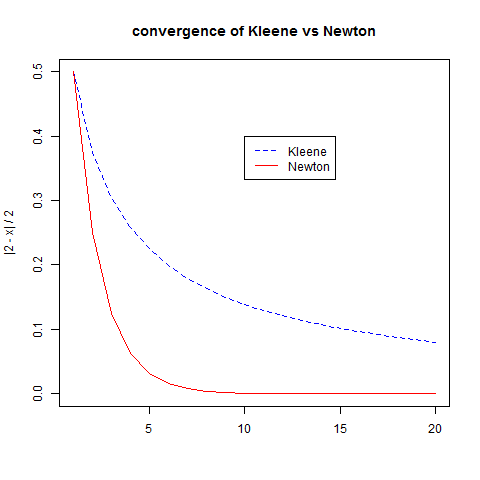
\includegraphics[width=100mm]{fig/k-n.png}
		\end{center}
		\caption{Kleene法とNewton法の収束スピード}
		\label{fig:cKleene法とNewton法の収束スピード}
	\end{figure} %}
%s3:逐次近似たち}

\subsubsection{導出木}\label{s3:導出木} %{
	形式言語の場合と同様に、cc-半環に対しても導出木を定義する。
	\cite{EKL07}にある部分導出木の定義はよくわからないが、次のようなものだろう。
	\begin{equation*}\begin{split}
		x = a + bx^2
		\sim x + \xymatrix@R=4pt@C=4pt{
			x \hen[d] \\ a
		} + \xymatrix@R=4pt@C=4pt{
			& x \hen[ld] \hen[d] \hen[rd] \\
			b & x & x \\
		} + \xymatrix@R=4pt@C=4pt{
			& x \hen[ld] \hen[d] \hen[rd] \\
			b & x \hen[d] & x \\
			& a \\
		} + \xymatrix@R=4pt@C=4pt{
			& x \hen[ld] \hen[d] \hen[rd] \\
			b & x \hen[ld] \hen[d] \hen[rd] & x \\
			b & x & x \\
		} + \cdots
	\end{split}\end{equation*}
	そして、すべての葉のラベルが$\set{a,b}$の場合、導出木と定義している。
	導出木は次のようにして通常の導出過程に関係している。
	\begin{equation*}\begin{split}
		\xymatrix@R=6pt{
			& & bax \ar@{=>}[rd] \\
			x \ar@{=>}[r] & bxx \ar@{=>}[ru] \ar@{=>}[rd] && baa \\
			& & bxa \ar@{=>}[ru] \\
		}\sim \xymatrix@R=4pt@C=4pt{
			& x \hen[ld] \hen[d] \hen[rd] \\
			b & x \hen[d] & x \hen[d] \\
			& a & a \\
		}
	\end{split}\end{equation*}

	\cite{EKL07}では、木の次元を定義して、その次元を用いて逐次近似の収束性を
	を議論している。ただし、同様のことを行っている同じ筆者達の
	\cite{DBLP:confcalcoEsparzaL11}では、木の次元の定義が異なっている。
	正直、\cite{EKL07}の定義は破綻している気がする。ここでは、木の次元を
	\cite{DBLP:confcalcoEsparzaL11}によって定義しておく。
	\begin{equation*}\begin{split}
		\dim\bullet := 1 \\
		\dim\word{t_1,\dots,t_n} = \begin{cases}
			d + 1, &\text{ if } d = \dim t_i \text{となる$i$が二つ以上ある} \\
			d, &\text{ otherwise } \\
		\end{cases} \\
		\quad\text{where } d := \max_{i=1}^n\dim t_i
	\end{split}\end{equation*}
	このように木の次元を定義する理由は、\cite{DBLP:confcalcoEsparzaL11}に
	次のように書いてある。
	`` Recall that Kleene’s approximation corresponds to evaluating the derivation trees
of G by increasing height. The question whether we can charaterize Newton’s approximation
in a similar way has been answered positively in [EKL10]. We need the notion
of dimension of a derivation tree.''
	木の次元は次のようになる。
	\begin{equation*}\begin{split}
		\xymatrix@R=4pt@C=4pt{
			& x:2 \hen[ld] \hen[d] \hen[rd] \\
			b:1 & x:1 \hen[d] & x:1 \hen[d] \\
			& a:1 & a:1 \\
		},\quad \xymatrix@R=4pt@C=4pt{
			& x:2 \hen[ld] \hen[d] \hen[rd] \\
			b:1 & x:2 \hen[ld] \hen[d] \hen[rd] & x:1 \hen[rd] \\
			b:1 & a:1 & a:1 & a:1 \\
		},\quad \xymatrix@R=4pt@C=4pt{
			& x:2 \hen[ld] \hen[d] \hen[rd] \\
			b:1 & x:2 \hen[ld] \hen[d] \hen[rd] & x:1 \hen[rd] \\
			b:1 & x:2 \hen[ld] \hen[d] \hen[rd] & a:1 & a:1 \\
			b:1 & a:1 & a:1 \\
		}
	\end{split}\end{equation*}
%s3:導出木}
\subsubsection{証明たち}\label{s3:証明たち} %{
	\begin{proposition}[Taylorの定理]\label{prop:Taylorの定理} %{
		$R$をcc-半環とする。
		任意の$\plr{f\bou x}\in R\bblr{x}$と$y\in R$に対して次の不等式が
		成り立つ。
		\begin{equation*}\begin{split}
			\plr{f\bou x} + \plr{\partial f\bou x}y \le \plr{f\bou x + y}
			\le \plr{f\bou x} + \plr{\partial f\bou x + y}y
		\end{split}\end{equation*}
	\end{proposition} %prop:Taylorの定理}
	\begin{proof} %{
		まず、$R\blr{x}$が$x$で生成されることを用いて、多項式に対して
		命題の不等式が成り立つことを証明する。
		\begin{itemize}\setlength{\itemsep}{-1mm} %{
			\item $\plr{f\bou x}=a\in R$の時
			\begin{equation*}\begin{split}
				\plr{f\bou x} + \plr{\partial f\bou x}y = \plr{f\bou x + y}
				= \plr{f\bou x} + \plr{\partial f\bou x + y}y = a
			\end{split}\end{equation*}
			\item $\plr{f\bou x}=x$の時
			\begin{equation*}\begin{split}
				\plr{f\bou x} + \plr{\partial f\bou x}y = \plr{f\bou x + y}
				= \plr{f\bou x} + \plr{\partial f\bou x + y}y = x + y
			\end{split}\end{equation*}
			\item $\plr{f\bou x}=\plr{g\bou x} + \plr{h\bou x}$の時 \\
			多項式の項数についての帰納法で証明する。
			\begin{equation*}\begin{split}
				\plr{f\bou x + y} &= \plr{g\bou x + y} + \plr{h\bou x + y} \\
				&\ge \plr{g\bou x} + \plr{\partial g\bou x}y
					+ \plr{h\bou x} + \plr{\partial h\bou x}y \\
				&= \plr{f\bou x} + \plr{\partial f\bou x}y \\
				%
				\plr{f\bou x + y} &= \plr{g\bou x + y} + \plr{h\bou x + y} \\
				&\le \plr{g\bou x} + \plr{\partial g\bou x + y}y
					+ \plr{h\bou x} + \plr{\partial h\bou x + y}y \\
				&= \plr{f\bou x} + \plr{\partial f\bou x + y}y \\
			\end{split}\end{equation*}
			\item $\plr{f\bou x}=\plr{g\bou x}\plr{h\bou x}$の時 \\
			多項式の次数についての帰納法で証明する。
			$y$の二次の項を捨てることで次の式が成り立つことがわかる。
			\begin{equation*}\begin{split}
				\plr{f\bou x + y} &= \plr{g\bou x + y}\plr{h\bou x + y} \\
				&\ge \plrgg{\plr{g\bou x} + \plr{\partial g\bou x}y}
					\plrgg{\plr{h\bou x} + \plr{\partial h\bou x}y} \\
				&\ge \plr{g\bou x}\plr{h\bou x}
					+ \plrgg{\plr{\partial g\bou x}\plr{h\bou x} 
					+ \plr{g\bou x}\plr{\partial h\bou x}}y \\
				&= \plr{f\bou x} + \plr{\partial f\bou x}y
			\end{split}\end{equation*}
			また、$\plr{g\bou x}\le\plr{g\bou x + y}$により、次の式が成り立つ
			ことがわかる。
			\begin{equation*}\begin{split}
				\plr{f\bou x + y} &= \plr{g\bou x + y}\plr{h\bou x + y} \\
				&\le \plrgg{\plr{g\bou x} + \plr{\partial g\bou x + y}y}
					\plr{h\bou x + y} \\
				&= \plr{g\bou x}\plr{h\bou x + y} 
					+ \plr{\partial g\bou x + y}\plr{h\bou x + y}y \\
				&= \plr{g\bou x}\plr{h\bou x} + \plrgg{
					\plr{g\bou x}\plr{\partial h\bou x + y}
					+ \plr{\partial g\bou x + y}\plr{h\bou x + y}}y \\
				&\le \plr{g\bou x}\plr{h\bou x} + \plrgg{
					\plr{g\bou x + y}\plr{\partial h\bou x + y}
					+ \plr{\partial g\bou x + y}\plr{h\bou x + y}}y \\
				&= \plr{f\bou x} + \plr{\partial f\bou x + y}y
			\end{split}\end{equation*}
		\end{itemize} %}
		次に、可算個の多項式の和によって任意の形式級数を書くことが
		できるとして($\omega$-連続の定義)、形式級数に対して証明する。
	\end{proof} %}

	\begin{proposition}[Taylorの定理(ベキ等)]\label{prop:Taylorの定理(ベキ等)} %{
		$R$をベキ等なcc-半環とする。
		任意の$\plr{f\bou x}\in R\bblr{x}$と$y\in R$に対して次の式が成り立つ。
		\begin{equation*}\begin{split}
			\plr{f\bou x + y} = \plr{f\bou x} + \plr{\partial f\bou x + y}y
		\end{split}\end{equation*}
	\end{proposition} %prop:Taylorの定理(ベキ等)}
	\begin{proof} %{
		ベキ等半環では、任意の$n\in\sizen$に対して次の式が成り立つ。
		\begin{equation*}\begin{split}
			\plr{x+y}^{n+1} = \sum_{k=0}^{n+1} x^ky^{n+1-k}
			= x^{n+1} + y\sum_{k=0}^n x^ky^{n-k}
			= x^{n+1} + y\plr{x+y}^n
		\end{split}\end{equation*}
		したがって、任意の単項式に対して命題が成り立つ。
		そして、係数環が$\omega$-連続だから、単項式の無限和に対しても命題が
		成り立つ。
	\end{proof} %}
%s3:証明たち}
%s1:EKL07}
}\endgroup %}
